% ****** Start of file apssamp.tex ******
%
%   This file is part of the APS files in the REVTeX 4 distribution.
%   Version 4.0 of REVTeX, August 2001
%
%   Copyright (c) 2001 The American Physical Society.
%
%   See the REVTeX 4 README file for restrictions and more information.
%
% TeX'ing this file requires that you have AMS-LaTeX 2.0 installed
% as well as the rest of the prerequisites for REVTeX 4.0
%
%
%\documentclass[preprint,amsmath,amssymb]{revtex4}
%\documentclass[prd,amsmath,amssymb]{revtex4}
% use this for PRL/PRD, add "preprint" to get double space
%\documentclass[prd,twocolumn,showpcs,amsmath,amssymb]{revtex4}

%\documentclass[aps,prd,twocolumn,superscriptaddress,showpacs]{revtex4}
\documentclass[aps,prd,onecolumn,superscriptaddress,showpacs]{revtex4}


%%%%%%%%%%% To get line numbers: %%%%%%%%%%%%%%%
%\documentclass[12pt,twoside,letterpaper,doublespace]{article}%
%\topmargin -0.25cm
%\textwidth 15.5cm
%\textheight 22cm
%\oddsidemargin 0.5cm
%\evensidemargin 0.5cm%

%%%%%%%%%%%%%%%%%%%%%%%%%%%%%%%%%%%%%%%



\usepackage{graphicx}% Include figure files
\usepackage{dcolumn}% Align table columns on decimal point
%\usepackage{bm}% bold math
\usepackage{epsfig,amssymb}



%%%%%%%%%%% To get line numbers: %%%%%%%%%%%%%%%

%\usepackage{lineno}
%\usepackage{setspace}

%%%%%%%%%%%%%%%%%%%%%%%%%%%%%%%%%%%%%%%




\input phys_def.tex

\setlength{\topmargin}{-15mm}
% \fontfamily{ptm}\selectfont\renewcommand{\rmdefault}{ptm}
% \usepackage{mathptmx}
\begin{document}

%\begin{flushright}
%{\large\bf DRAFT 3.0}\\
%\end{flushright}

% remove the following for publication
%\begin{figure}
%\leftline{\includegraphics[scale=0.5]{cdfii_thumb_logo.eps}\hfill
%CDF note 7398}
%\end{figure}
% remove the space for publication
%\vspace*{1.5cm}

\title{
{\large\bf
 Search for NMSSM Higgs $h \to aa \to \mu \mu \mu \mu$      
}
%\\ \vspace*{2.0cm}
}



%\affiliation{URL http://www-cdf.fnal.gov}

\date{\today}
%\maketitle


\begin{abstract}
% remove the space for publication
%\vspace*{3.0cm}

We present a study ... 

%\vspace*{5.0cm} \centerline{\em Preliminary Results for Winter 2005 Conferences}
\end{abstract}

% activate the following line for publication
\pacs{13.38.Dg 13.38.Qk}

\maketitle

%%%%%%%%%%%%%%%%%%%%%%% End of latex definitions %%%%%%%%%%%%%%%%%%%%%%%
%
%%%% Stuff to get line numbering: %%%%%%%%%%%%%%%
%\pagewiselinenumbers
%\doublespace






%\newpage

%%%%%%%%%%%%%%%%%%%%%%%%%%%%%%%%%%%%%%%%%%%%%%%%%%%%%%%%%%%%%%%%%%%%%%%%%%%
% Introduction 
%

\section{Introduction}

Tension between the electroweak data fits preferance for light higgs and limits
from direct searches can be resolved by an elegant solution handed by the NMSSM. 
A possible solution could be that there is a new mode for higgs decay $h \to aa$,
where $a$ is a pseudoscalar higgs field, thus diminishing the branching ratios for
conventional modes used in direct higgs searches and largely softening direct higgs
mass limits from LEP. While `naturalness' and `fine tuning' arguments have lead to
somewhat extensive studies of the region of masses of $a$ above $\tau \tau$ and $b\bar{b}$ 
threshold, the results require a substantial integrated luminosity and are technically
very challenging analysis. 

At the same time, the region of lower masses (below $2 m_\tau$) has not been studied. We 
propose here an analysis targeting the range of $m_a$ below the $\tau \tau$ threshold by 
exploring the decay $h \to aa \mu \mu \mu \mu$. Unlike searches with taus, the two muon mass
gives a direct estimate of $m_a$ providing a substantially better constrained system. 
Further, this channel is essentially free of backgrounds and therefore one can use
direct gluon fusion production instead of smaller vector boson fusion process that has
to be used in order to suppress large QCD backgrounds. 

{\bf Current constraints in this region come from XXX and are fairly weak - need SASHA's help here}.

We show that the analysis in
the four muon mode has excellent sensitivity for higgs and can be performed with just 
a handful of first CMS data and requires very little in terms of detector performance 
except reasonably robust tracking for muons and well functioning muon system. To make 
this a realistic analysis, we use parameters of the CMS experiment in designing
selections and estimating background contributions.


\section{NMSSM Parameter Space}

The allowed NMSSM parameter space permits at least two
phenomenologically-distinct Higgs systems, one in which a 120~GeV
scalar Higgs decays primarily into conventional $WW^*$, $b\bar{b}$,
and $\tau^+\tau^-$ modes, and another with a light, hidden Higgs that decays
almost exclusively into $aa$.  The latter has only been excluded up to
86~GeV by specialized searches at LEP (upper limit due to $e^+e^- \to
h Z$ kinematics)~\cite{lep1exclusion,lep2exclusion}, leaving the
86--120~GeV region unexplored (Fig~\ref{mass_exclusion}).

\begin{figure}[htb]
\begin{center}
\includegraphics[width=0.45\linewidth]{plots/mass_exclusion.eps}
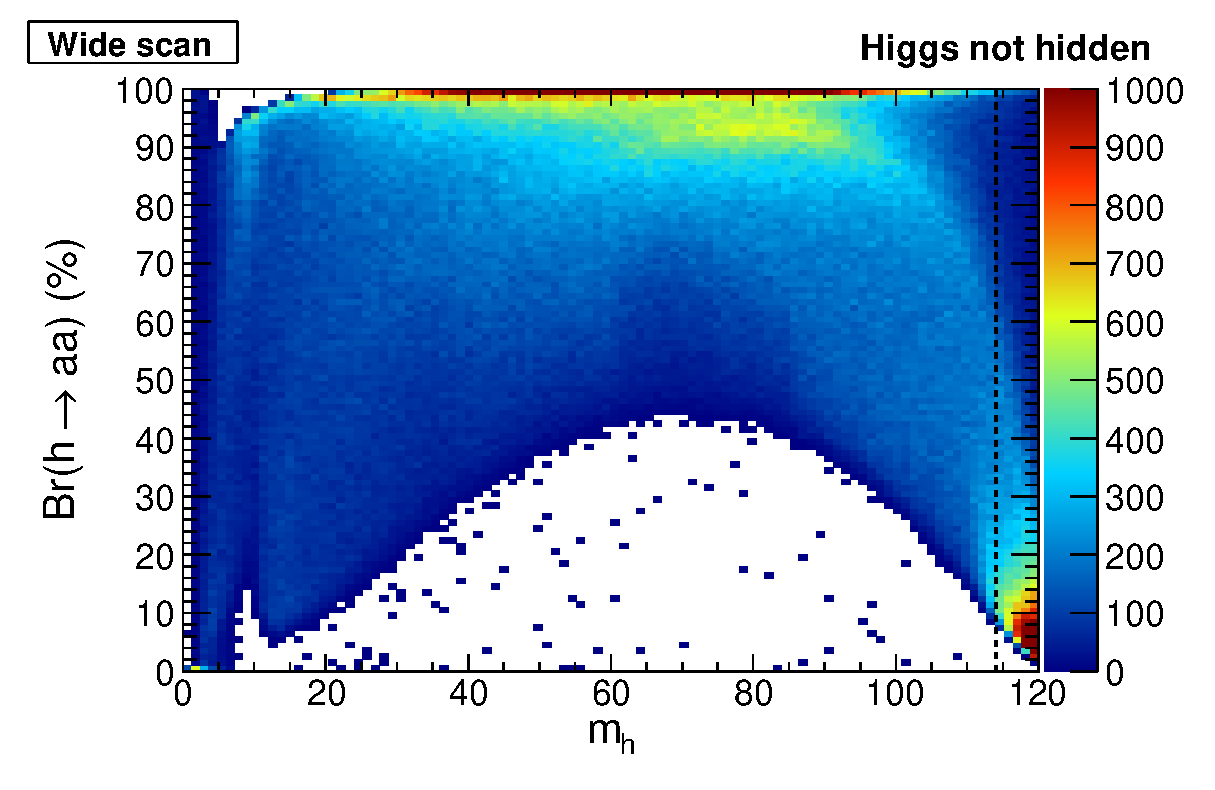
\includegraphics[width=0.45\linewidth]{plots/mh_brhaa.eps}
\caption{Left: regions of $m_a$ vs.\ $m_h$ excluded by LEP searches,
  right: the strong correlation between $m_h$ and $B_{h \to aa}$.  The above scan is subject to experimental constraints (other
  than the two specialized LEP searches for $h\to aa$) which require a
  conventionally-decaying Higgs to have $m_h >
  114$~GeV. \label{mass_exclusion}}
\end{center}
\end{figure}

We used the NMSSMTools
package~\cite{nmssmtools1,nmssmtools2,nmssmtools3} to scan the NMSSM
parameter space and to identify the region with $B_{h \to aa}
\gg B_{h \to WW^*\mbox{\scriptsize, } b\bar{b}\mbox{\scriptsize, }\tau^+\tau^-}$.
Scans are uniform in each parameter listed in Table~\ref{brhaa_table},
subject to phenomenological and experimental constraints except for
the specialized LEP $h\to aa$ searches.  Two scans were performed,
labeled ``wide'' and ``narrow,'' where the narrow scan focuses more
exclusively on the hidden Higgs region.  The $\lambda$ and $A_\kappa$
parameters are restricted even in the wide scan to yield small $m_a$
values, important for large $B_{a\to\mu\mu}$.  A particularly
important parameter for distinguishing between conventional Higgs
decays and hidden decays is the ratio of $\kappa$ over $\lambda$, so
we perform uniform scans in this ratio, rather than $\kappa$ alone.
Fig~\ref{brhaa_plots} shows how each parameter is related to
$B_{h \to aa}$.

\begin{table}[htb]
\caption{Ranges for NMSSM parameter scans.  The narrow scan focuses on
the region with high $B_{h \to aa}$. \label{brhaa_table}}
\begin{center}
\renewcommand{\arraystretch}{1.2}
\begin{tabular}{| c c |}
\hline \mbox{\hspace{1.25 cm}}Wide scan\mbox{\hspace{1.25 cm}} & \mbox{\hspace{1.25 cm}}Narrow scan\mbox{\hspace{1.25 cm}} \\\hline
$0 < \kappa/\lambda < 0.8$ & $0 < \kappa/\lambda < 0.5$ \\
$0 < \lambda < 0.1$ & {\it same} \\
$-0.1 < A_\kappa < 0$~GeV & {\it same} \\
$0 < A_\lambda < 4$~TeV & $1 < A_\lambda < 3$~TeV \\
$100 < \mu < 200$~GeV & $100 < \mu < 150$~GeV \\
$10 < \tan\beta < 60$ & $10 < \tan\beta < 33$ \\\hline
\end{tabular}
\end{center}
\end{table}

\begin{figure}[htb]
\begin{center}
\includegraphics[width=0.45\linewidth]{plots/pmass1_lambda.eps}
\includegraphics[width=0.45\linewidth]{plots/pmass1_Akappa.eps}

\caption{Both $\lambda$ and $A_\kappa$ must be close to zero for $m_a$
  to be below the $2 \, m_\tau$ threshold. \label{pmass1_Akappa}}
\end{center}
\end{figure}

\begin{figure}[htb]
\begin{center}
\includegraphics[width=0.45\linewidth]{plots/brhaa_koverl.eps}
\includegraphics[width=0.45\linewidth]{plots/brhaa_lambda.eps}

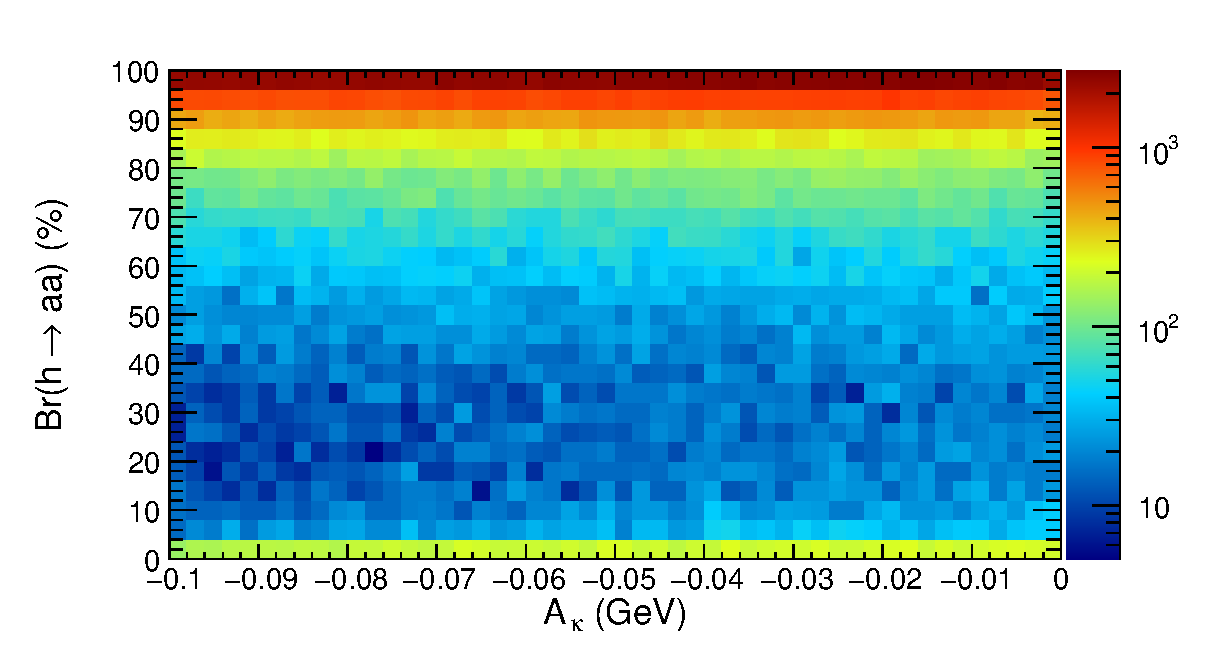
\includegraphics[width=0.45\linewidth]{plots/brhaa_Akappa.eps}
\includegraphics[width=0.45\linewidth]{plots/brhaa_Alambda.eps}

\includegraphics[width=0.45\linewidth]{plots/brhaa_mu.eps}
\includegraphics[width=0.45\linewidth]{plots/brhaa_tanbeta.eps}

\caption{$B_{h \to aa}$ as a function of each of the NMSSM
  parameters with dashed lines indicating the ``narrow scan'' cuts
  (Table~\ref{brhaa_table}).  All narrow scan cuts are applied except
  for the one shown.  Note the logarithmic color scale used to
  highlight the difference between $B_{h \to aa} \approx
  \mbox{0\%}$ and $\approx \mbox{100\%}$. \label{brhaa_plots}}
\end{center}
\end{figure}

To determine the sensitivity of our 4-muon search channel, we also
need to know the branching fraction of $a\to\mu\mu$.  In the mass
range of interest (below the $a \to \tau^+\tau^-$ threshold), the main
competing channels are $a \to gg$ and $a \to s\bar{s}$.  We again use
NMSSMTools to calculate these (with $m_s = 95$~MeV and no cut on
$m_a$), which are nearly a function of $m_a$ only.  The final
branching fractions are presented in Fig~\ref{brh4mu_plots}.

\begin{figure}
\begin{center}
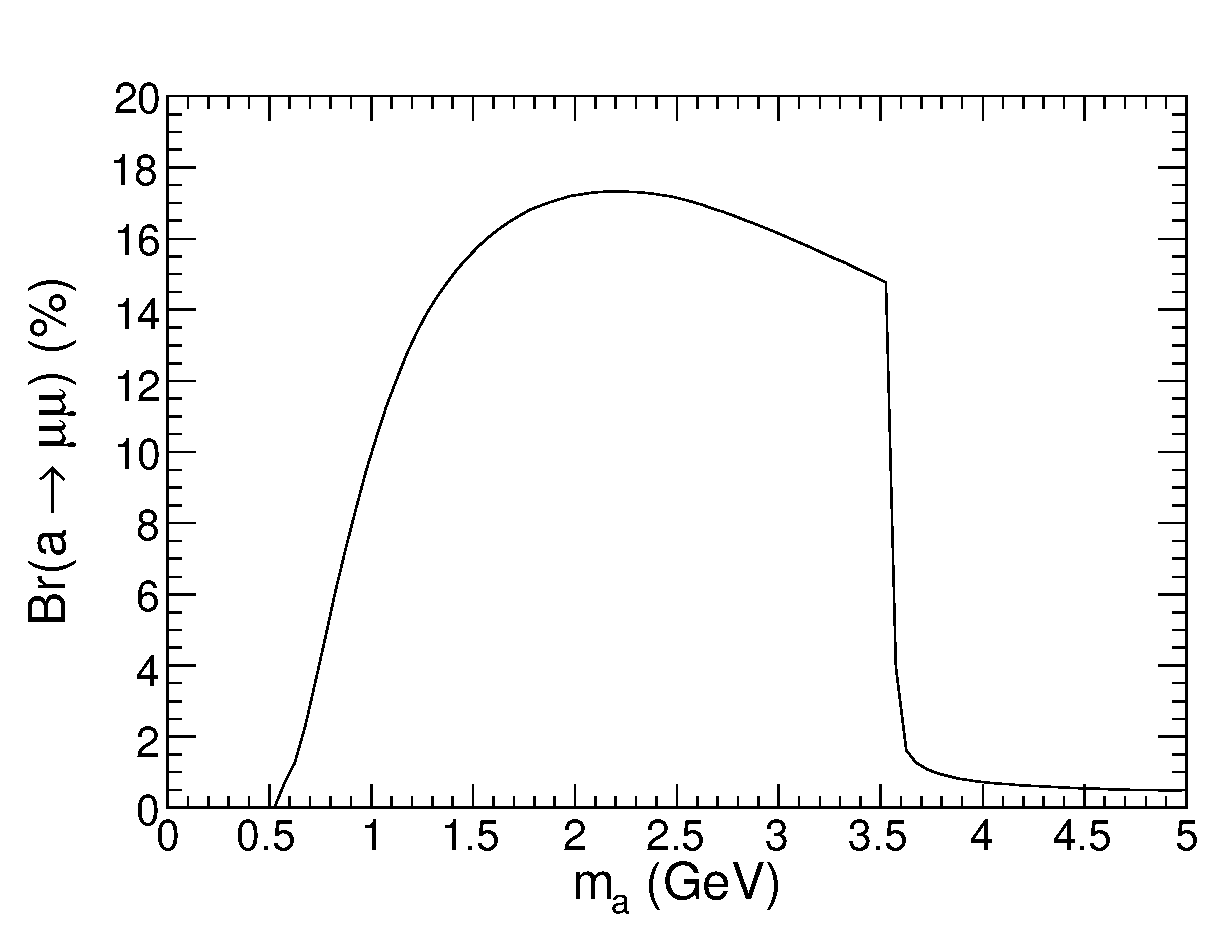
\includegraphics[width=0.31\linewidth]{plots/branching_fractions_plot.eps}
\includegraphics[width=0.31\linewidth]{plots/brh4mu_pmass1.eps}
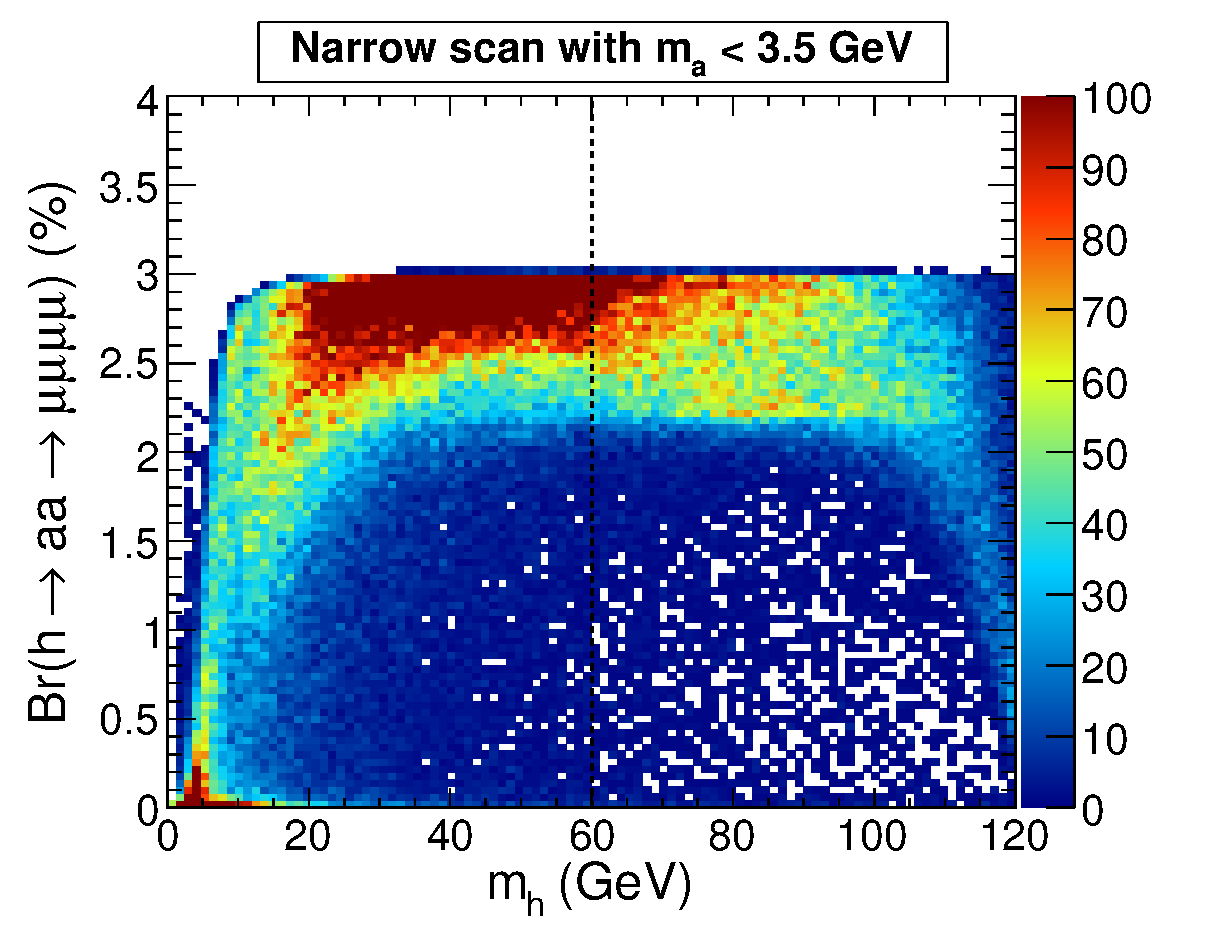
\includegraphics[width=0.31\linewidth]{plots/brh4mu_smass1.eps}
\caption{Branching fractions of $a \to \mu\mu$ and full $h \to aa \to \mu\mu\mu\mu$ chain
  as a function of $m_a$ and $m_h$. \label{brh4mu_plots}}
\end{center}
\end{figure}

\subsection{Production Cross Section $pp \to h + X$ }

Due to relatively low expected backgrounds in the case of the four muon channel,
one should go after the dominant production modes of higgs boson. We include $gg
\to h$ and $bb \to h$. The higgs production cross-section is calculated in the framework of NMSSM
for typical sets of parameters using XXX and YYY. Figure 2 shows the predicted
cross-section for several typical choices of parameters and also a comparison
with the Standard Model higgs production cross-section. {\bf Need Sasha to write this one!!!}

\section{Analysis}

The main characteristics of the anaysis are two back-to-back pairs of spatially 
close muons. Each of the di-muon pairs should have invariant mass consistent 
with $m_a$ and the four muon invariant mass should give a bump corresponding to
the higgs mass. We use these facts in designing an analysis with a reasonably
high acceptance and very low backgrounds suitable for early LHC running.

\subsection{Signal Simulation}
We used Pythia to generate signal events (should we give settings?). We
generated samples with $m_h \times m_a = (70, 80, 90, 100, 110, 120 \; GeV/c^2) \times
(1, 1.5, 2, 2.5, 3 \; GeV/c^2)$. We used XXX to emulate detector response (major
parameters are muon momentum resolution, low threshold on muons to reach 
the muon system, acceptance and average reconstruction efficiencies that were
taken from CMS TDR). 

Figure 3 and 4 show invariant masses of the muon pairs (we force correct assignment of pairs using generator
information) and of the 4 muon system.

\begin{figure}[htb]
\begin{center}
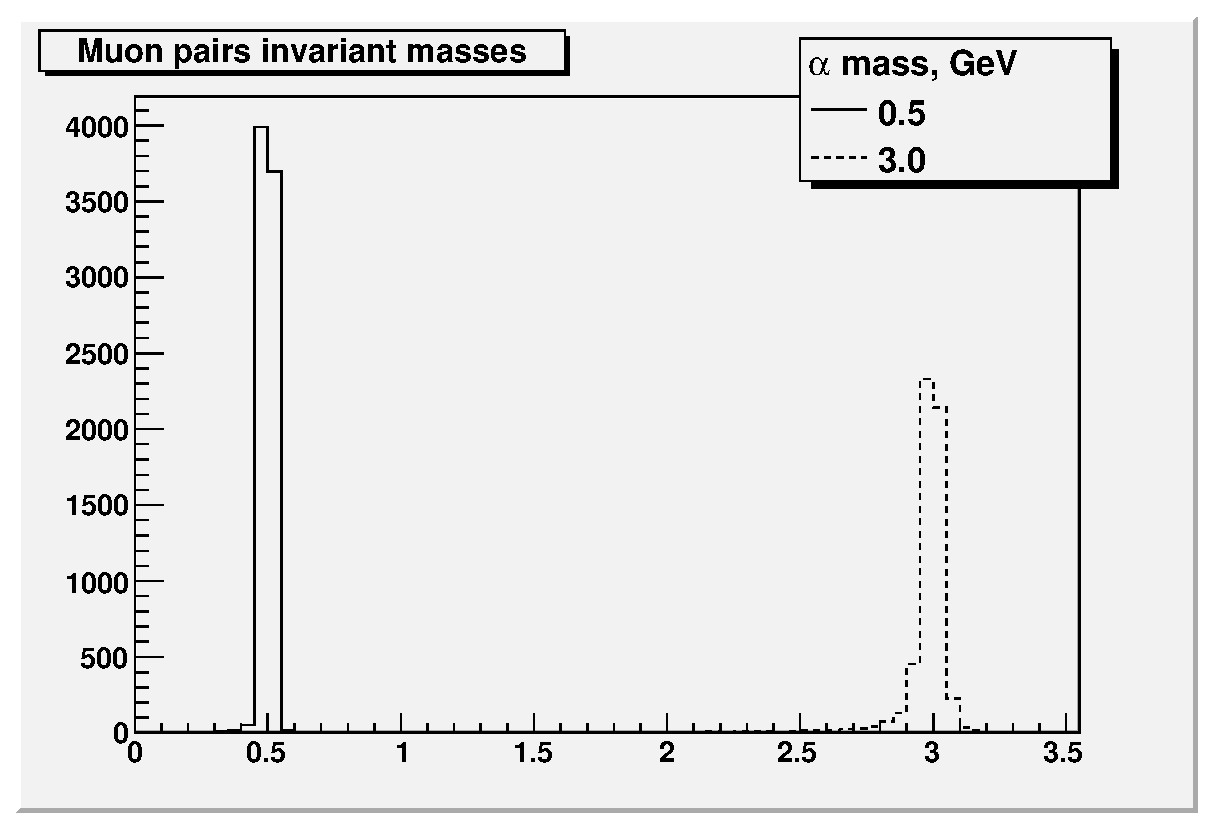
\includegraphics[width=15pc]{plots/muon_pairs_masses.eps}
\caption{Muon pairs invariant masses ($m_H$ = 100 GeV)}
\label{muon_pairs_masses}
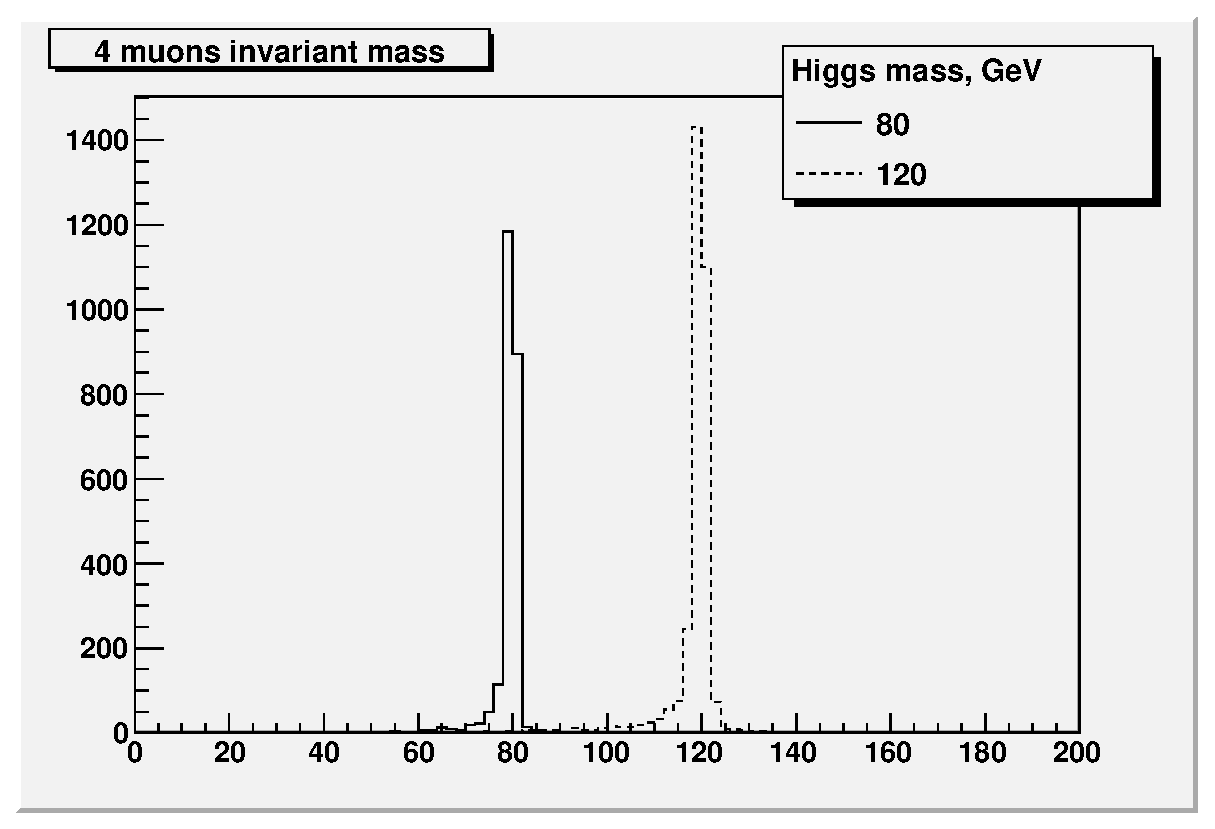
\includegraphics[width=15pc]{plots/invariant_mass.eps}
\caption{4 muons invariant mass ($m_a$ = 3.0 GeV)}
\label{invariant_mass}
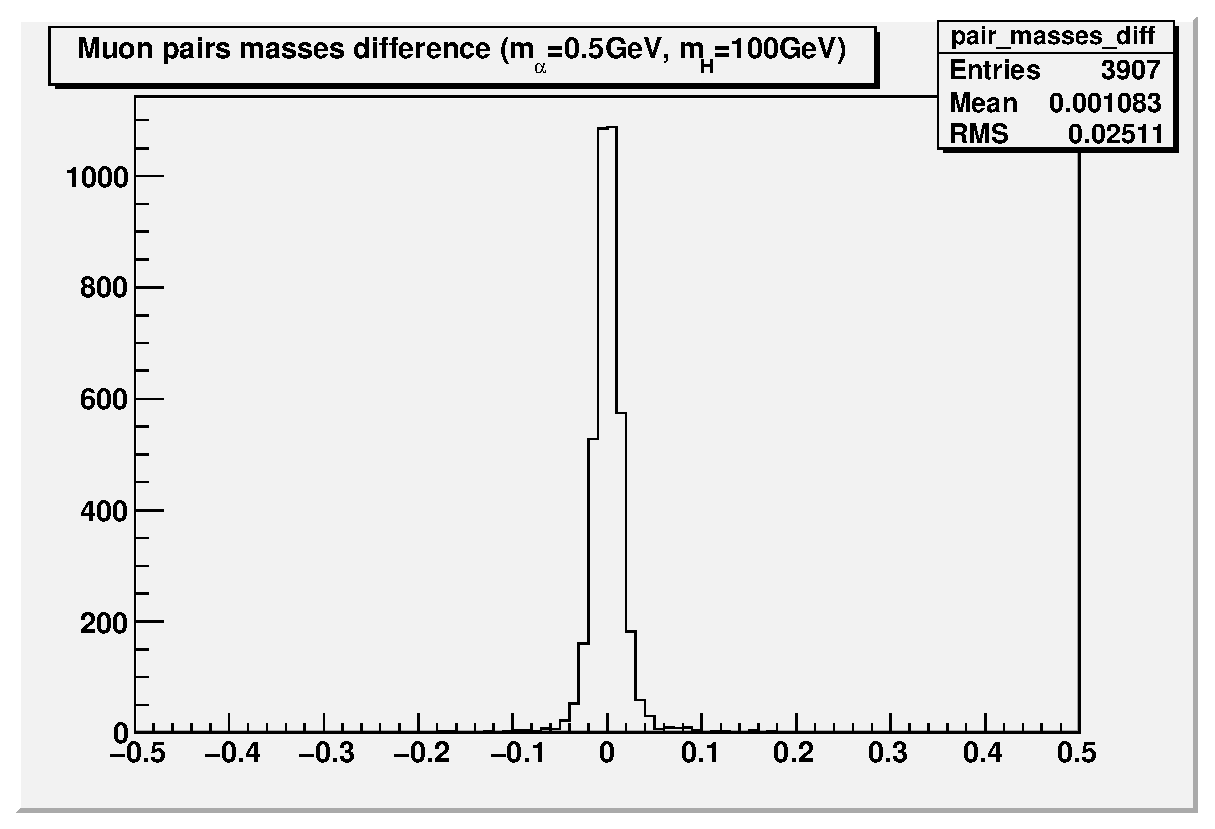
\includegraphics[width=15pc]{plots/pairs_masses_diff_0.5.eps}
\caption{Muon pairs masses difference ($m_a$=0.5GeV, $m_H$=100 GeV)}
\label{muon_pairs_masses_diff_0.5}
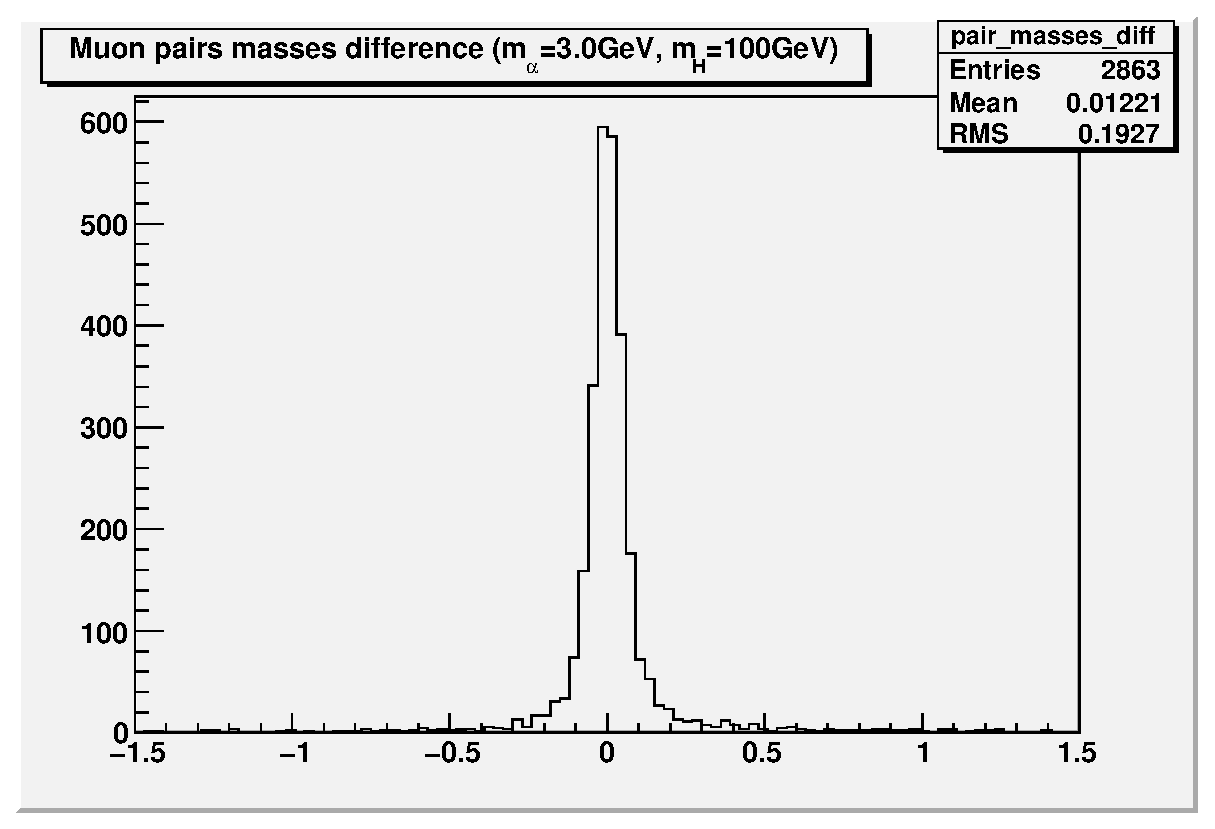
\includegraphics[width=15pc]{plots/pairs_masses_diff_3.0.eps}
\caption{Muon pairs masses difference ($m_a$=3.0GeV, $m_H$=100 GeV)}
\label{muon_pairs_masses_diff_3.0}
\end{center}
\end{figure}


\subsection{Event Reconstruction}
The analysis starts by requiring at least four muon candidates with $p_T>5$ \gevc in the fiducial volume of the
detector. At least one of the four muons has to have $p_T>20$ \gevc to satisfy likely trigger requirements. Each
event must have at least two muon candidates of positive and negative charge. In events satisfying these 
critiria, we define quadruplets of candidates consisting of two positive and two negatively charged muon
candidates. Note that at this point there could be more than one quadruplet per event, e.g. if there are 
five muons in the event. 

At the next step, inside each quadruplet, we sort out the four muon candidates into two pairs (pairs will 
later beassociated to one of the two axial bosons $a$). We perform this assignment by requiring that in each pair
there must be two muon candidates of opposite charge and minimizing the $MIN_{(i,j,k,l)} (\Delta R(\mu_i,\mu_j)^2 + \Delta R (\mu_k,\mu_l)^2)$ 
to determine the most likely assignment of four muons into two pairs $(i,j)\bigoplus(k,l)$. {\bf Figure 5 shows the 
distribution for this value showing high efficiency of this algorithm for the range of $(m_h, m_a)$ values of interest 
to this analysis.} At his point muon candidates are assigned into pairs and invariant mass of each of the pair (we denote the pair masses 
as $m_{12} and m_{34}$) is calculated as well as invariant mass of all four muons, we denote it as $m_{1234}$ or $M$. 
Fig. \ref{figX1} shows the distribution of invariant masses of such pairs for signal events with $(m_h,m_a)=(90,0.5)$ 
\gevcc (solid line) and $(m_h,m_a)=(90,2.5)$ \gevcc that passed all previous selections. Figure \ref{figX2} shows the distribution of 
the four muon invariant mass, M, for signal events generated with $(m_h,m_a)=(70,1.5)$ (solid line) and $(120, 1.5)$ \gevcc (dashed line).

{\bf We consider adding isolation requirements to muons to decrease the fraction of the muons originating from jets.
That should go along the lines of what we discussed earlier (isolation of the pair, not individual muons).}

The kinematics of signal events and the specific interest of this analysis in the region of $0.5<m_a<3.6$, $m_h>60$ \gevcc, one could
reasonably apply additional selections on $m_{12}$, $m_{34}$, $m_{1234}$ and $|m_{12}-m_{34}|$ (to enforce the requirement that the
two pair masses are consistent with each other). We choose to keep all remaining events and instead develop a fitting procedure that 
works in a 3D space $(m_{12},m_{34}, m_{1234})$ that is aware of special kinematical properties of signal events (they will appear as 
a bump in one specific small region in this 3D space). Our approach allows preserving all available acceptance and maximize statistical 
power of the analysis. It is also convenient from experimental point of view as the backgrounds will be distributed in some smooth 
fashion over the 3D space allowing fitting the 3D distribution to estimate backgrounds directly from the data.

{\bf Acceptance for these cuts is shown in Table \ref{acceptance}. Note Figures \ref{acceptance_H} and \ref{acceptance_a} show acceptance as a 
function of $m_h$ for several fixed $m_a$ and as a function of $m_a$ for several choices of $m_h$ values. - we should recalculate acceptances
corresponding to this point, currently they are quoted for after the next series of `illustrational' cuts}.

However, to give reader a better idea of the signal and background rates in the region consistent with the signal kinematics and the target
region of this analysis, we also quote overall acceptance (and later background efficiencies and rates) for the following cuts as if they
were applied after the main cuts above: both pair reconstructed mass values, $m_{12}$ and $m_{34}$, should be less than 4 \gevcc; the invariant
mass of the four muons $m_{1234}>$60 \gevcc; and $|m_{12}-m_{34}|<X$ \gevcc. 

{\bf we need to add plots for pair mass ($m_{12},m_{34}$, $m_{1234}$, $m_{12}-m_{34}$.}

\begin{figure}[htb]
\begin{center}
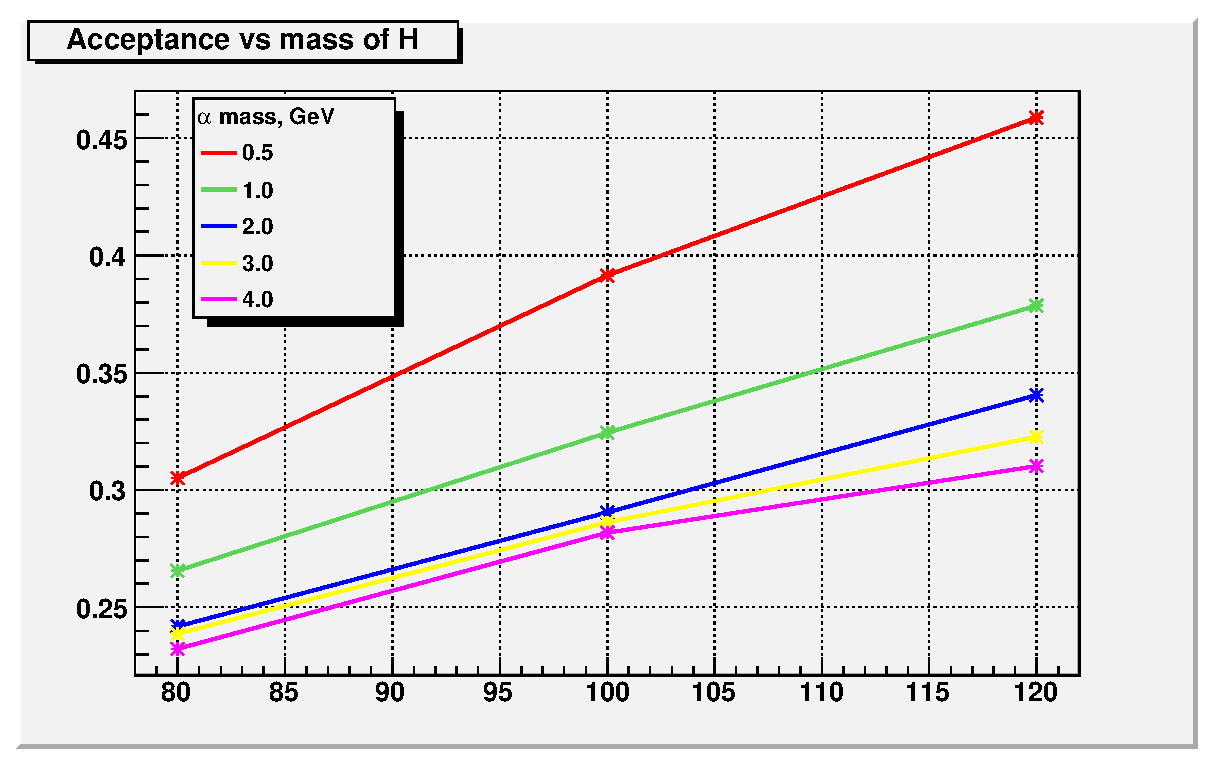
\includegraphics[width=15pc]{plots/acceptance_H.eps}
\caption{Acceptance as a function of $m_h$ for fixed $m_a$}
\label{acceptance_H}
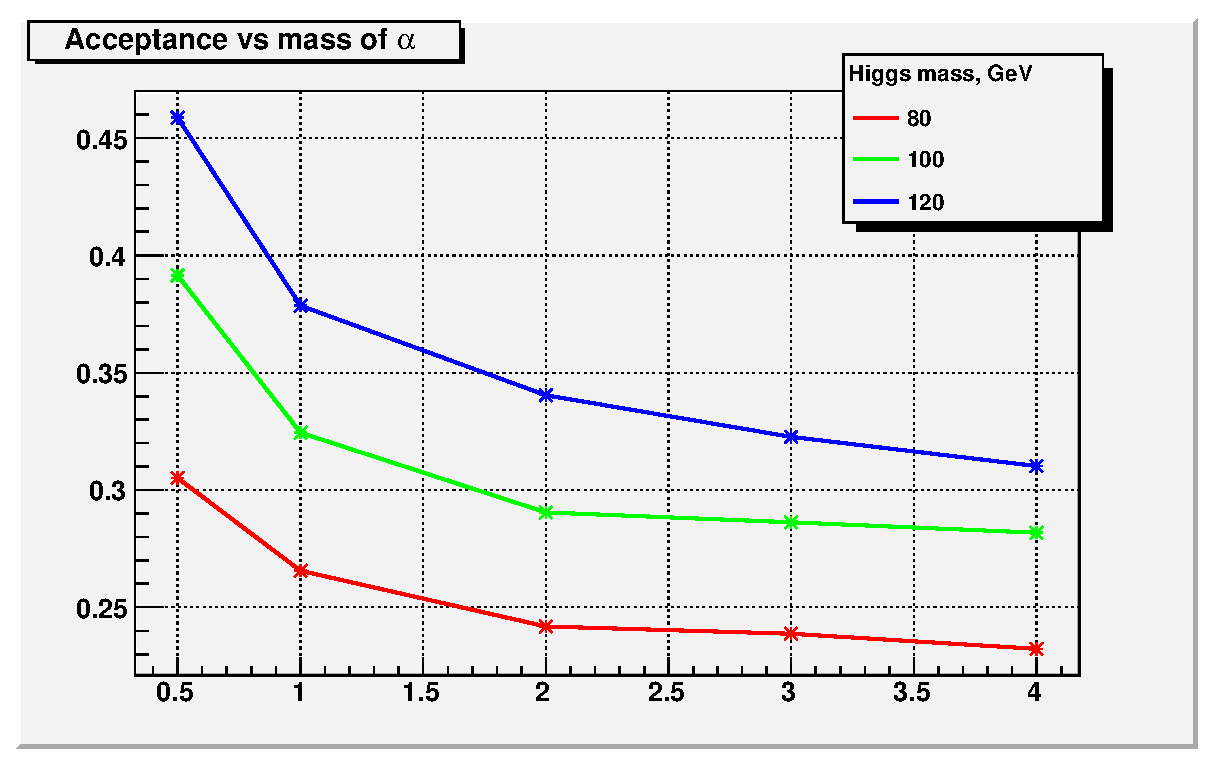
\includegraphics[width=15pc]{plots/acceptance_a.eps}
\caption{Acceptance as a function of $m_a$ for fixed $m_h$}
\label{acceptance_a}
\end{center}
\end{figure}

%\begin{figure}[htb]
%\begin{center}
%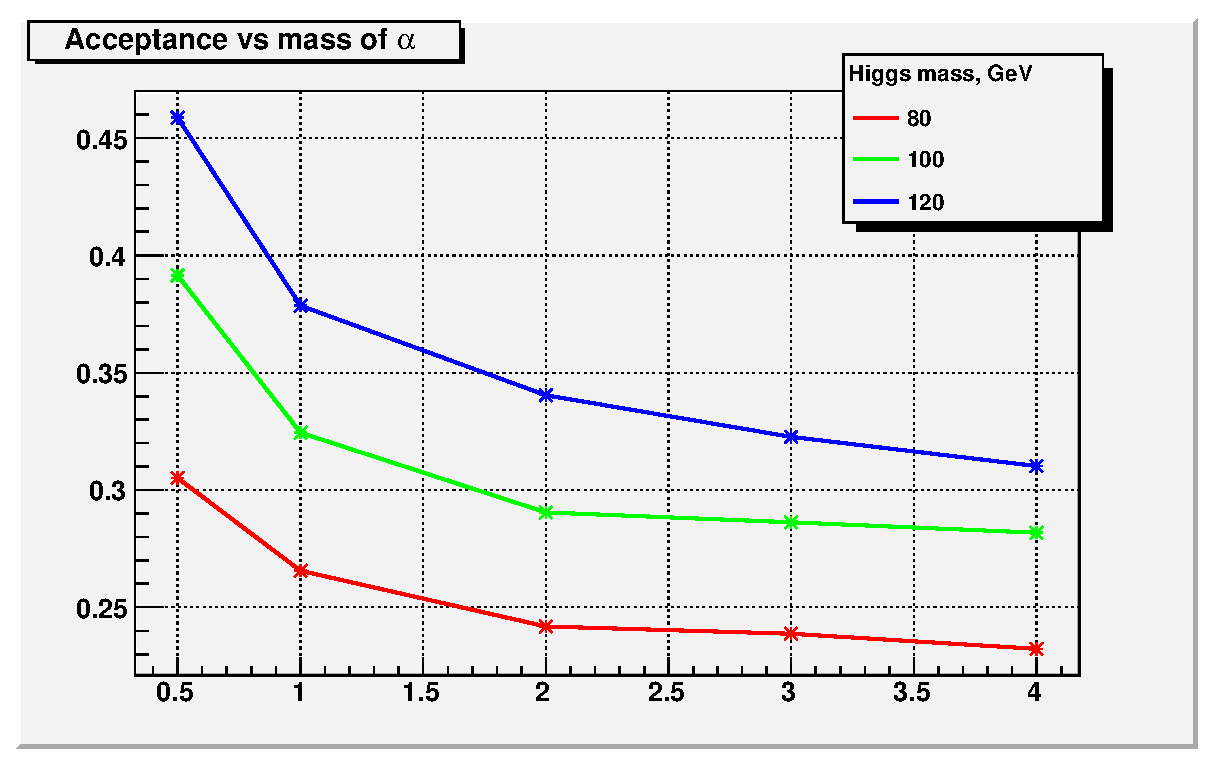
\includegraphics[width=15pc]{plots/acceptance_a.eps}
%\caption{Acceptance as a function of $m_a$ for fixed $m_h$}
%\label{acceptance_a}
%\end{center}
%\end{figure}


Table \ref{acceptance} shows acceptances for different points in $m_h$-$m_a$ space.

\begin{table}[t]
\caption{Acceptances for various points in $m_h$-$m_a$ space.\label{acceptance}}
\begin{center}
\begin{tabular}{|c|c|c|c|c|c|}
\hline
%\multicolumn{3}{|c|}{hey}\\ \hline
$m_h$, $m_a$ (GeV) & 0.5 & 1.0 &2.0&3.0&4.0\\ \hline
80&    $0.3052\pm0.0046$    &    $0.2656\pm0.0044$    &    $0.2420\pm0.0043$    &    $0.2389\pm0.0043$    &    $0.2324\pm0.0043$    \\ \hline
100&   $0.3915\pm0.0049$    &    $0.3245\pm0.0047$    &    $0.2906\pm0.0045$    &    $0.2862\pm0.0045$    &    $0.2819\pm0.0045$    \\ \hline
120&   $0.4587\pm0.0050$    &    $0.3785\pm0.0049$    &    $0.3405\pm0.0047$    &    $0.3226\pm0.0047$    &    $0.3103\pm0.0046$    \\ \hline
\end{tabular}
\end{center}
\end{table}




\subsection{Background Estimation}

\subsubsection{QCD backgrounds}
Requirement of four muons in the event selection drastically reduces contributions of background
processes. The largest contribution comes from rare QCD events where four real muons are produced 
in heavy flavor decays of b and c mesons. This background can be substantially reduced by the 
requirement of at least one muon with $p_T>20$ GeV/c and can be estimated using Pythia Monte Carlo. 
Another QCD background comes from events with two or three real muons from heavy flavor decays and 
the remaining candidates come from misidentification dominated by $K/\pi$ decays in flight. This
background can be estimated using the same Pythia sample by selecting events with two or three 
real muons and a charged pion or kaon satisfying $p_T$ and $\eta$ requirements used in this analysis 
for muons and weighing such combinations with the probability to decay into a muon before reaching 
radius of $\simeq$2 meters. We find that the level of backgrounds due to misidentifications is 
comparable to the rate of the backgrounds associated with real muons from heavy flavor decays. 
However, both of these contributions are further suprpessed by the requirement of the four muon invariant
mass to be above 60 GeV and a requirement that pairs of such muons have low invariant mass. While
the fraction of remaining events at this point is still not negligible, the probability that muon 
candidates in background events can be arranged in pairs of similar invariant masses is very small 
making QCD contributions nearly negligible. One can essentially completely eliminate these backgrounds 
by applying loose track isolation requirement on each of the pairs.

We used Pythia Monte Carlo to simulate four muon QCD backgrounds using $2 \to 2$ 
QCD production where we required at least one muon (either real from e.g. b or c
quark decays or from pion and kaon decays in flight) with transverse 
momentum above 20 $GeV/c$ (to be consistent with the definition of
non-isolated inclusive muon trigger at CMS). In addition, we generated a large 
sample of $J/\psi$ events. Other SM backgrounds (ZZ*, top) were foudn to be 
small in the mass region of interest. Figure 7 and 8 show the same distributions
as in Figures 3 and 4, but for the signal + SM backgrounds overlayed. Note that 
these plots are not reflective of the true significance of signal over background 
because these plots do not take into account that the two pair masses must be 
consistent with each other and simultaneously form a narrow peak in the four muon 
mass.

\subsubsection{$J/\psi$}

We also studied direct $J/\psi$ production process that can produce a pair of muons with mass in
the range of interest of this analysis and another pair of muons can come from decays in flight. We
used Pythia MC and a weighing technique similar to the QCD case and find that this background is
completely negligible.

\subsubsection{Electroweak four lepton backgrounds}

We use CompHEP to generate a large sample of events with four muons in final state coming from electroweak 
processes. The cross-section of this process is 0.5 pb ({\bf Sasha, is this correct? Kind of sounds very 
small!!!}) and after a cut on the first muon $p_T>20$ GeV/c, the large chunk of remaining events are 
$Z\gamma^*$ type events. Very few of these events have muons that can be arranged into pairs with low invariant 
mass, and the fraction of events with similar masses of the pairs is completely negligible.

\subsubsection{Summary}
While the number of events going into the final fit is not small, the fitting procedure described in the next
section is effectively reducing the region of interest to events that have similar invariant masses of the 
two pais of muons, which leaves us in essentially zero background situation. Tables \ref{bckgr_cuts_efficiency_gen_level,bckgr_cuts_efficiency_reco_level,bckgr_cuts_number_gen_level,bckgr_cuts_number_reco_level}
show efficiency of passing
sequential cuts for each type of backgrouns as well as the number of expected background events after each cut in a 
dataset corresponding to 100 \ipb of LHC data.

\begin{table}[t]
\caption{Background cuts efficiency for generator level\label{bckgr_cuts_efficiency_gen_level}}
\begin{center}
\begin{tabular}{|c|c|c|c|}
\hline
%\multicolumn{3}{|c|}{hey}\\ \hline
Cuts & 4 leptons & $\mu+x$ & $J/\Psi$ \\ \hline
1st eta$<$2.4&                 $0.7994\pm0.0040$    &    $0.95638\pm0.00073$       &    $0.0088\pm0.0022$   \\ 
2nd eta$<$2.4&                 $0.8295\pm0.0042$    &    $0.99992\pm0.00003$       &    $1.00^{+0.00}_{-0.06}$ \\ 
3rd eta$<$2.4&                 $0.8541\pm0.0044$    &    $0.99584\pm0.00024$       &    $0.75\pm0.11$       \\ 
4th eta$<$2.4&                 $0.7066\pm0.0061$    &    $0.96407\pm0.00068$       &    $0.75\pm0.13$       \\ 
1st pt$>$5&                    $0.9805\pm0.0022$    &    $1.00000^{+0}_{-0.00001}$ &    $1.0^{+0.0}_{-0.1}$   \\ 
2nd pt$>$5&                    $0.9405\pm0.0038$    &    $0.8676\pm0.0013$         &    $1.0^{+0.0}_{-0.1}$   \\ 
3rd pt$>$5&                    $0.7893\pm0.0068$    &    $0.0445\pm0.0008$         &    $0.3333\pm0.1571$   \\ 
4th pt$>$5&                    $0.4390\pm0.0093$    &    $0.0284\pm0.0032$         &    $0.00^{+0.27}_{-0.00}$  \\ 
1st pt$>$20&                   $0.9524\pm0.0060$    &    $0.9873\pm0.0126$         &    $0$    \\ \hline
analysis acceptance &          $0.1218\pm0.0033$    &    $0.00099\pm0.00011$       &    $0$    \\ \hline
pair masses$<$4&               $0.0025\pm0.0014$    &    $0.3333\pm0.0533$         &    $0$    \\ 
inv. mass$>$60 &               $0.6667\pm0.3333$    &    $0.4231\pm0.0969$         &    $0$    \\ 
$|m_{12}-m_{34}|<$X GeV &      $X.XXXX\pm X.XXXX$    &    $X.XXXX\pm X.XXXX$         &    $0$    \\ \hline
full efficiency&            $0.000203\pm0.000143$&    $0.00014\pm0.00004$       &    $0$    \\ \hline
\end{tabular}
\end{center}
\end{table}

\begin{table}[t]
\caption{Background cuts efficiency for reco level\label{bckgr_cuts_efficiency_reco_level}}
\begin{center}
\begin{tabular}{|c|c|c|c|}
\hline
%\multicolumn{3}{|c|}{hey}\\ \hline
Cuts & 4 leptons & $\mu+x$  & $J/\Psi$ \\ 
\hline
1st pt$>$5&                    $0.7455\pm0.0044$    &    $1.00000^{+0}_{-0.00001}$   &    $1.0000^{+0}_{-0.0006}$ \\ 
2nd pt$>$5&                    $0.7012\pm0.0053$    &    $1.00000^{+0}_{-0.00001}$   &    $1.0000^{+0}_{-0.0006}$ \\ 
3rd pt$>$5&                    $0.6066\pm0.0068$    &    $0.04349\pm0.0007$          &    $0.3333\pm0.0013$       \\ 
4th pt$>$5&                    $0.3300\pm0.0084$    &    $0.0402\pm0.0034$           &    $0.00^{+0.15}_{-0.00}$  \\ 
1st pt$>$20&                   $0.9573\pm0.0063$    &    $1.000^{+0}_{-0.007}$       &    $0$    \\ 
\hline
analysis acceptance &          $0.1002\pm0.0030$    &    $0.0017\pm0.0002$         &    $0$    \\ 
\hline
pair masses$<$4&               $0.0041\pm0.0020$    &    $0.3358\pm0.0403$           &    $0$    \\ 
inv. mass$>$60 &               $0.50\pm0.25$        &    $0.4348\pm0.0731$           &    $0$    \\ 
$|m_{12}-m_{34}|<$X GeV &      $X.XXXX\pm X.XXXX$    &    $X.XXXX\pm X.XXXX$         &    $0$    \\ 
\hline
full efficiency&               $0.00020\pm0.00014$  &    $0.00025\pm0.00006$         &    $0$    \\ 
\hline
\end{tabular}
\end{center}
\end{table}



\begin{table}[t]
\caption{Number of events after each selection cut on generator level\label{bckgr_cuts_number_gen_level}}
\begin{center}
\begin{tabular}{|c|c|c|c|}
\hline
%\multicolumn{3}{|c|}{hey}\\ \hline
Cuts & 4 leptons & Incl. muon & JPsi \\ 
\hline
Initial number&            $48.21\pm0.49$    &    $152878.11\pm546.06$    &    $120.91\pm2.84$   \\ 
1st eta$<$2.4&             $38.54\pm0.43$    &    $146209.61\pm534.01$    &    $1.0652\pm0.2663$ \\ 
2nd eta$<$2.4&             $31.97\pm0.40$    &    $146197.91\pm533.99$    &    $1.0652\pm0.2663$ \\ 
3rd eta$<$2.4&             $27.30\pm0.37$    &    $145589.38\pm532.88$    &    $0.7989\pm0.2306$ \\ 
4th eta$<$2.4&             $19.29\pm0.31$    &    $140358.34\pm523.22$    &    $0.5992\pm0.1997$ \\ 
1st pt$>$5&                $18.92\pm0.30$    &    $140358.34\pm523.22$    &    $0.5992\pm0.1997$ \\ 
2nd pt$>$5&                $17.79\pm0.30$    &    $121774.70\pm487.35$    &    $0.5992\pm0.1997$ \\ 
3rd pt$>$5&                $14.04\pm0.26$    &    $5424.13\pm102.86$      &    $0.1997\pm0.1153$ \\ 
4th pt$>$5&                $6.17\pm0.17$     &    $154.08\pm17.34$        &    $0$      \\ 
1st pt$>$20&               $5.87\pm0.17$     &    $152.13\pm17.23$        &    $0$      \\ 
\hline
pair masses$<$4&           $0.0147\pm0.0085$ &    $50.71\pm9.95$          &    $0$      \\ 
inv. mass$>$60 &           $0.0098\pm0.0069$ &    $21.45\pm6.47$          &    $0$      \\ 
$|m_{12}-m_{34}|<$X GeV &  $X.XXXX\pm X.XXXX$ &    $X.XXXX\pm X.XXXX$       &    $0$    \\ 
\hline
\end{tabular}
\end{center}
\end{table}

\begin{table}[t]
\caption{Number of events after each selection cut on reco level\label{bckgr_cuts_number_reco_level}}
\begin{center}
\begin{tabular}{|c|c|c|c|}
\hline
%\multicolumn{3}{|c|}{hey}\\ \hline
Cuts & 4 leptons & Incl. muon & JPsi \\ 
\hline
Initial number&            $48.21\pm0.49$    &    $152878.11\pm546.06$    &    $120.91\pm2.84$   \\ 
1st pt$>$5&                $35.94\pm0.42$    &    $152878.11\pm546.06$    &    $120.91\pm2.84$   \\ 
2nd pt$>$5&                $21.20\pm0.35$    &    $152878.11\pm546.06$    &    $0.3995\pm0.1631$ \\ 
3rd pt$>$5&                $15.29\pm0.27$    &    $6648.99\pm113.88$      &    $0$      \\ 
4th pt$>$5&                $5.04\pm0.16$     &    $267.21\pm22.83$        &    $0$      \\ 
1st pt$>$20&               $4.83\pm0.15$     &    $267.21\pm22.83$        &    $0$      \\ 
\hline
pair masses$<$4&           $0.0049\pm0.0098$ &    $89.72\pm13.23$         &    $0$      \\ 
inv. mass$>$60 &           $0.0098\pm0.0069$ &    $39.01\pm8.72$          &    $0$      \\ 
$|m_{12}-m_{34}|<$X GeV &  $X.XXXX\pm X.XXXX$ &    $X.XXXX\pm X.XXXX$       &    $0$    \\ 
\hline
\end{tabular}
\end{center}
\end{table}




\section{Statistical Analysis of the Data}

To maximize sensitivity and emulate real data analysis techniques, we define a likelihood function in the 3D space 
$(m_{pair \; 1}, \; m_{pair \; 2}, M)$, where M is the four muon invariant mass. The likelihood is defined as follows:
\begin{eqnarray}
{\cal L}(m_h, m_a, \sigma(pp \to h)) = \prod_i {\cal P}(\sigma(pp \to h) L B_{h \to aa} B^2_{a \to \mu \mu} L
\alpha(m_h, m_a) S_i (m_a, m_h) + L B_i, N^D_i)
\end{eqnarray}
where $i$ runs over bins in 3D space of $(m_{12}, m_{34}, m_{1234})$, $m_h$ is light higgs mass, $m_a$ is 
axial mass, ${\cal P}(\nu, N)$ is Poisson probability for observing $N$ events when the true rate is $\nu$, $L$ 
is luminosity, $\alpha$ is acceptance of the signal events, $S_i$ is the fraction of reconstructed signal events 
in bin $i$, $B_i$ is the rate of background events in bin $i$ per unit of luminosity.

We have studied QCD background events in the Monte Carlo and found that their distribution in the $(m_{12}, m_{34}, M)$ space can be
parameterized the following function:
\begin{eqnarray}
B(m_{12}, m_{34}, m_{1234}) = f(m_12) \times f(m_34) \times g(m_{1234}). 
\end{eqnarray}
Parameters of the function are shown in Table \ref{table_background_fit_parameters} and were obtained by fitting
the distribution of invariant masses of pairs. Note that in the analysis we randomly assign pairs of muons as `first' 
or `second' pair to ensure they have the same distribution. We verified that background events found in MC are well 
described by this function by running pseudoexperiments using paramaterized distribution and verifying that the p-value
for the outcome similar to what is observed in MC is high.

\subsection{Exclusion Levels if No Excess Observed}

Thus defined, the likelihood function is sufficient to calculate the
95\% C.L.\ exclusion region in $(m_a, m_h)$ parameter space.  We run
pseudoexperiments with background only (no signal) to calculate the
95\% C.L.\ on the product $\sigma(pp \to h) B_{h \to aa} B^2_{a \to \mu \mu} \, \alpha$,
which is 0.0293~pb at $L = 100$~pb$^{-1}$,
approximately 3 events.  This result is independent of $m_h$ and $m_a$
because the effective signal region tested by the fitter is background
free.

Since $B_{a \to \mu\mu}$ is nearly a function of $m_a$ only, it can be
factored out, and the corresponding upper limit on $\sigma(pp \to h)
B_{h \to aa} \alpha$ is presented in
Table~\ref{table_bramumu_factorized}.  The upper limit on
$\sigma(pp \to h) B_{h \to aa}$ is shown as a function of $m_h$ and
$m_a$ in Table~\ref{table_both_factorized} by factoring out $\alpha$
as well.  Keep in mind that $B_{h \to aa}$ is close to 100\% in much
of our preferred region of NMSSM parameter space.

\begin{table}[htb]
\caption{95\% C.L.\ on $\sigma(pp \to h) B_{h \to aa} \, \alpha$ at $L = 100$~pb$^{-1}$ as a function of $m_a$, from Fig~\ref{brh4mu_plots}. \label{table_bramumu_factorized}}
\begin{center}
\renewcommand{\arraystretch}{1.1}
\begin{tabular}{| c | c | c |}
\hline
\mbox{\hspace{0.25 cm}}$m_a$ (GeV)\mbox{\hspace{0.25 cm}} & \mbox{\hspace{0.25 cm}}$B_{a \to \mu\mu}$ (\%)\mbox{\hspace{0.25 cm}} & \mbox{\hspace{0.25 cm}}$\sigma(pp \to h) B_{h \to aa} \, \alpha$ (pb)\mbox{\hspace{0.25 cm}} \\\hline
0.5 & 0 & $\infty$ \\
0.75 & 4.2 & 16.5 \\
1.0 & 10.0 & 2.9 \\
1.5 & 15.7 & 1.2 \\
2.0 & 17.2 & 1.0 \\
2.5 & 17.1 & 1.0 \\
3.0 & 16.1 & 1.1 \\
3.5 & 14.8 & 1.3 \\
3.75 & 1.02 & 282 \\
4.0 & 0.73 & 557 \\
5.0 & 0.49 & 1220 \\\hline
\end{tabular}
\end{center}
\end{table}

\begin{table}[htb]
\caption{95\% C.L.\ on $\sigma(pp \to h) B_{h \to aa}$ (pb) at $L = 100$~pb$^{-1}$, from Fig~\ref{brh4mu_plots} and Table~\ref{acceptance}. \label{table_both_factorized}}
\begin{center}
\renewcommand{\arraystretch}{1.3}
\begin{tabular}{| c | c | c | c | c | c |}
\hline
\mbox{\hspace{0.25 cm}}$m_h$, $m_a$ (GeV)\mbox{\hspace{0.25 cm}} & \mbox{\hspace{0.25 cm}}0.5\mbox{\hspace{0.25 cm}} & \mbox{\hspace{0.25 cm}}1.0\mbox{\hspace{0.25 cm}} & \mbox{\hspace{0.25 cm}}2.0\mbox{\hspace{0.25 cm}} & \mbox{\hspace{0.25 cm}}3.0\mbox{\hspace{0.25 cm}} & \mbox{\hspace{0.25 cm}}4.0\mbox{\hspace{0.25 cm}} \\\hline
80 & $\infty$ & 10.9 & 4.1 & 4.6 & 2400 \\\hline
100 & $\infty$ & 8.9 & 3.4 & 3.8 & 2000 \\\hline
120 & $\infty$ & 7.7 & 2.9 & 3.4 & 1800 \\\hline
\end{tabular}
\end{center}
\end{table}

\subsection{Discovery Levels if Excess Observed}

Figure \ref{plots/likelihood_H100_a3_10pb.eps} shows results of a pseudoexperiment in which pseudodata was a combination 
of background events and signal with $\sigma (pp \to H)$=10 \ipb, $B(H \to aa \to \mu \mu \mu \mu)$=0.04, $m_a=3$ GeV, 
$m_h= 100$ GeV. The plot shows likelihood function ${\cal L}(m_h, m_a, \sigma(pp \to h))$ vs $\sigma(pp \to h)$ for 
$m_h$ and $m_a$ set to the true values. It is clear that significance of such signal is very large.

However, in real experiment, one does not look at fixed values of $m_a$ and $m_h$. Instead, one scans likelihood function
searching for an overall maximum in the $m_a,m_h,\sigma (pp \to H)$ space. Probability of oberving an excess of certain 
significance due to background fluctuation anywhere in the range is much larger than observing it in any a priori chosen 
point in $m_a,m_h$, therefore significance has to be corrected to account for the fact that we essentially run many searches 
at the same time. 

Rather then attempting to obtain `trial factor' analytically, the practical solution is to calculate the p-value, which is 
the probability of observing a fake signal from background fluctuation as significant as the one seen in data anywhere 
in the range analyzed in the measurement.

For simplicity we choose to scan data using a 2D grid in $(m_h \times m_a) = (60 - 200) \times (0.1, 4.0)$ with a step of 
3 GeV in $m_h$ direction and 0.1 GeV in $m_a$ direction. These values are chosen to be small enough to not miss a likely
signal.

To obtain smooth lines between the points in 
which signal samples were generated, we interpolated $S_i(m_h, m_a) = (S_i(m_h^j, m_a^j) + S_i(m_h^j+1,
m_a^j+1))/2$, where $j$ refers to nearest generated sample with lower masses, $j+1$ to the nearest sample with
hhigher masses.

\begin{figure}[htb]
\begin{center}
\includegraphics[width=15pc]{plots/likelihood_NoSignal.eps}
\caption{Example likelihood for a pseudoexperiment for a search assuming $B(H \to aa \to \mu \mu \mu \mu)$=0.04, 
$m_a=3$ GeV, $m_h= 100$ GeV with null signal shows that a 95\% exclusion is somewhere around 2.5 pb for  
$\sigma (pp \to H)$.}
\label{likelihood_null}
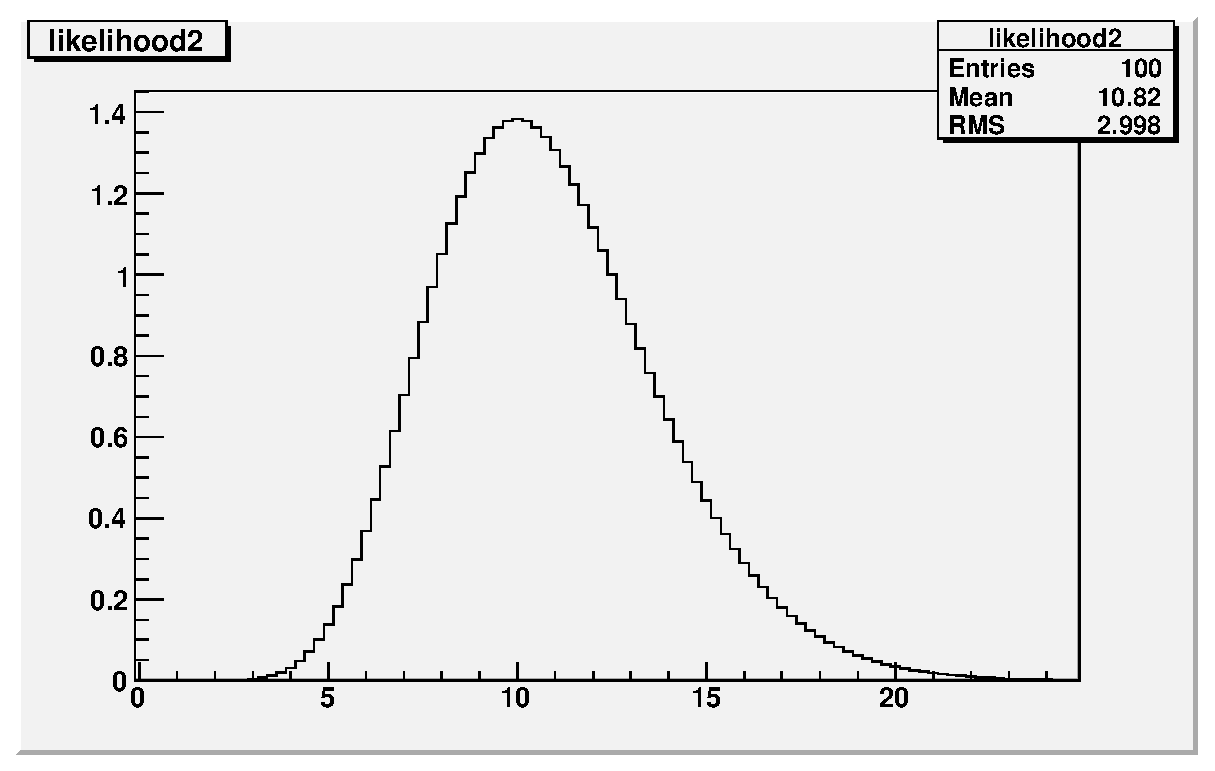
\includegraphics[width=15pc]{plots/likelihood_H100_a3_10pb.eps}
\caption{Example likelihood for $\sigma (pp \to H)$=10 \ipb, $B(H \to aa \to \mu \mu \mu \mu)$=0.04, $m_a=3$ GeV 
$m_h= 100$ GeV shows a more than $5 \sigma$ observation.}
\label{likelihood_10pb}
\end{center}
\end{figure}


\section{Results}

{\bf TO BE WRITTEN}

 




%
\section*{Acknowledgments}
We thank XXX and YYY

%\clearpage
%
%  References
%

%%%%%%%%%%%%%%%%%%%%%%%%%%%% References section %%%%%%%%%%%%%%%%%%%%%%%%%%
% A useful Journal macro
\def\Journal#1#2#3#4{{#1} {\bf #2}, #3 (#4)}
% Some useful journal names
\def\NCA{Nuovo Cimento}
\def\NIM{Nucl. Instrum. Methods}
\def\NIMA{{Nucl. Instrum. Methods} A}
\def\NP{Nucl. Phys.} 
\def\NPB{{Nucl. Phys.} B}
\def\PLB{{Phys. Lett.}  B}
\def\PRL{Phys. Rev. Lett.}
\def\RPP{Rep. Prog. Phys.}
\def\PRD{{Phys. Rev.} D}
\def\PR{Phys. Rep.}
\def\PRP{Prog. Theor. Phys.}
\def\ZPC{{Z. Phys.} C}
\def\MPL{{Mod. Phys. Lett.} A}
\def\EPJC{{Eur. Phys. J.} C}
\def\CPC{Comput. Phys. Commun.}

\renewcommand{\baselinestretch}{1}
%\mytableorig

\begin{thebibliography}{99}

%
% CDF detector
%
\bibitem{ua1-z} C.~Albajar~\etal  (UA1 Collaboration),  \Journal{\PLB}{253}{503}{1991};
J.~Alitti~\etal  (UA2 Collaboration),  \Journal{\PLB}{276}{365}{1992}.
\bibitem{lep-wz} The LEP Collaborations: ALEPH, DELPHI, L3 and OPAL, the LEP Electroweak Working Group and the SLD Electroweak
and Heavy Flavor Working Group (2004), hep-ex/0412015.
\bibitem{cdf-d0-z} T.~Affolder~\etal (CDF Collaboration), \Journal{\PRL}{84}{845}{2000}; 
F.~Abe~\etal  (CDF Collaboration), \Journal{\PRD}{59}{052002}{1999}; 
S.~Abachi~\etal  (D$\O$ Collaboration), \Journal{\PRL}{75}{1456}{1995}; 
B.~Abbot~\etal {} (D$\O$ Collaboration), \Journal{\PRD}{60}{053003}{1999}. 
\bibitem{w-z-e} D.~Acosta~\etal  (CDF Collaboration), \Journal{\PRL}{94}{091803}{2005};
A.~Abulencia~\etal (CDF Collaboration), FERMILAB-PUB-05-360 (2005), Submitted to Phys. Rev. D. 
\bibitem{D0_ztt} V.M.~Abazov~\etal (D$\O$ Collaboration), \Journal{\PRD}{71}{072004}{2005}.
\bibitem{run2_susy_higgs_workshop} M.~Carena~\etal, hep-ph/0010338; M.~Carena~\etal, \Journal{\EPJC}{26}{601}{2003}; S.~Abel~\etal, hep-ph/0003154.
\bibitem{belyaev} S. Belyaev, T. Han, and R. Rosenfeld, \Journal{JHEP}{0307}{021}{2003}.
\bibitem{susy_golden_mode} A.~Dedes~\etal, hep-ph/0207026.
\bibitem{CDFditauAnalyses} A. Abulencia~\etal (CDF Collaboration), \Journal{\PRL}{96}{011802}{2006}; 
D.~Acosta~\etal (CDF Collaboration), \Journal{\PRL}{95}{131801}{2005} .
\bibitem{CDFrunIhiggs} D. Acosta~\etal (CDF Collaboration), \Journal{\PRD}{72}{072004}{2005}. 
\bibitem{CDFDetector}  D. Acosta {\em et al.} (CDF Collaboration), \Journal{\PRD}{71}{032001}{2005}.
\bibitem{lt} S. Baroiant~\etal, \Journal{\NIMA}{518}{609}{2004}.
\bibitem{CDFLuminosity} S. Klimenko, J. Konigsberg, and T.M. Liss, FERMILAB-FN-0741 (2003). 
\bibitem{pythia} T. Sjostrand~\etal, \Journal{JHEP}{0207}{012}{2002}.
\bibitem{CTEQ6} J. Pumplin~\etal, \Journal{\CPC}{135}{238}{2001}.
\bibitem{D-track_reco} D.~Acosta~\etal (CDF Collaboration), \Journal{\PRL}{91}{241904}{2003}.
\bibitem{jet-energy-paper} A. Bhatti~\etal, \Journal{\NIMA}{566}{375}{2006}.
\bibitem{jet-clu} F. Abe~\etal (CDF Collaboration), \Journal{\PRD}{45}{1448}{1992}.
\bibitem{PDG} Particle Data Group, \Journal{\PLB}{592}{1}{2004}.
\bibitem{nnlo-x-sec} P. Sutton, A. Martin, R. Roberts, and W. Stirling, \Journal{\PRD}{45}{2349}{1992};
R. Rijken and W. van Neerven, \Journal{\PRD}{51}{44}{1995};
R. Hamberg, W. van Neerven, and T. Matsuura, \Journal{\NPB}{359}{343}{1991};
R. Harlander and W. Kilgore, \Journal{\PRL}{88}{201801}{2002};
W. van Neerven and E. Zijstra, \Journal{\NPB}{382}{11}{1992}.
\bibitem{cor-factor-zgamma} A. Martin, R. Roberts, W. Stirling, and R. S. Thorne, \Journal{\EPJC}{28}{455}{2003}.
\bibitem{geant} R.Brun~\etal, GEANT Detector Description and Simulation Tool, CERN Program Library, W5013, 1994.

% Jim's papers to be merged in
\bibitem{lep1exclusion} G.~Abbiendi~\etal (OPAL Collaboration), \Journal{\EPJC}{18}{425-445}{2001}.
\bibitem{lep2exclusion} G.~Abbiendi~\etal (OPAL Collaboration), \Journal{\EPJC}{27}{483-495}{2003}, arXiv:0209068v1 [hep-ex].
\bibitem{nmssmtools1} U.~Ellwanger, J.F.~Gunion and C.~Hugoine, \Journal{JHEP}{0502}{066}{2005}.
\bibitem{nmssmtools2} U.~Ellwanger, C.~Hugoine, \Journal{\CPC}{175}{290}{2006}.
\bibitem{nmssmtools3} F.~Domingo and U.~Ellwanger, arXiv:0710.3714 [hep-ph].




%
% Coordinate for CDF detector
%

%\bibitem{CDFdet} CDF Collaboration, F.~Abe~\etal, \Journal{\NIMA}{271}{387}{1988}.
    
%\bibitem{Topref} CDF Collaboration, F.~Abe~\etal, \Journal{\PRD}{50}{2966}{1994}.
\end{thebibliography}

\section{Appendix}


\begin{table}[t]
\caption{Background samples normalization\label{bckgr_normalize}}
\begin{center}
\begin{tabular}{|c|c|c|c|c|c|}
\hline
%\multicolumn{3}{|c|}{hey}\\ \hline
Sample & $\sigma$ & $N^{gen}_{evt}$ & Filter efficiency & $L_{eff}$ & $f = L_{100}/L_{eff}$ \\ \hline
$\mu+x$ &           $0.5091mb$    &    $6238383$      &    $0.000239$  &  $51.2709pb^{-1}$   &  $1.9504$ \\ \hline
4 leptons &        $0.538pb$     &    $10995$        &    $1.0$       &  $20436.803pb^{-1}$ &  $0.0049$ \\ \hline
$J/\psi$ &         $0.127.2nb$   &    $1413803$      &    $0.0074$    &  $1502.00pb^{-1}$   &  $0.0666$ \\ \hline

\end{tabular}
\end{center}
\end{table}

\end{document}
